\chapter{Prijedlog rješenja}
\paragraph*{}
U skladu sa datim zahtjevima predložena je izrada aplikacijske platforme pod nazivom Logit (
\gls{LAPP}), opisane u nastavku, sa detaljnim tehničkim detaljima u narednim poglavljima. Uzimajući u obzir data ograničenja, te funkcionalne i nefunkcionalne zahtjeve određeno je da se korisnička aplikacija izradi na Android platformi sa podrškom za Android API nivo počevši od nivoa 19 (4.4 KitKat), to je najniži nivo koji omogućava korištenja naprednih NFC i kriptografskih funkcionalnosti te osigurava dobru pokrivenost potencijalne korisničke baze sa ukupnom adopcijom od preko 90\% za navedenu ili višu verziju\cite{droidstats}. Za uspješan rad aplikacije neophodno je da korisnički uređaj podržava i NFC funkcionalnosti, prema prognozama analitičke kuće IHS Technology, do 2020. godine svaki treći uređaj imati će podršku za NFC.\cite{nfcforecast}

\section{Logički model rješenja}
\paragraph*{}
Priloženi dijagrami interakcije osnovnih funkcionalnosti Logit platforme i pripadajući opis imaju za cilj stvoriti opštu sliku sistema, te tako olakšati praćenje tehničkog modela rješenja datog u nastavku. Tehnički model opisuje dosta detaljniju sliku funkcioniranja sistema i može služiti kao svojevrstan uvod u kod platforme.

\subsection*{Registracija korisnika}
\begin{figure}[H]
    \centering
    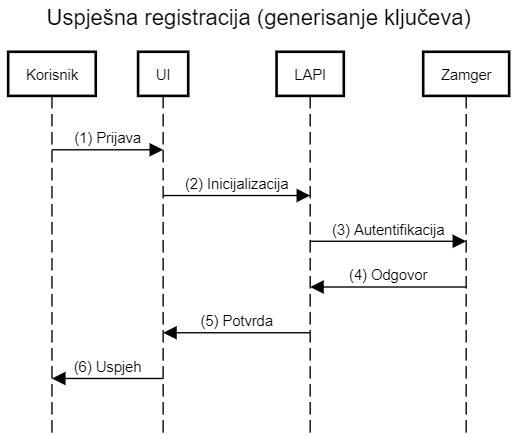
\includegraphics[width=0.7\textwidth]{material/dia/01_registracija}
    \caption{Dijagram interakcije - uspješna registracija i generisanje ključeva}
\end{figure}
\paragraph*{}
Nakon uspješne instalacije aplikacije na korisnički Android uređaj (DEVICE) potrebno je obaviti proces registracije koji se izvršava u dva bitna koraka. Prvi korak sastoji se od unosa već postojećih autentifikacijskih podataka za ZAMGER sistem Elektrotehničkog fakulteta, korisnik se korištenjem datih podataka posredstvom LAPI servisa autentificira na ZAMGER sistemu, bitno je napomenuti da Logit platforma ne sprema korisničku lozinku ZAMGER sistema, navedeni podaci se koriste isključivo za povezivanje postojećeg identiteta i novogenerisanog para korisničkih RSA ključeva (KEYS), što je ujedno i drugi korak u procesu registracije na Logit platformu.

\paragraph*{}
U slučaju uspješnje autentifikacije, korisnika se obavještava o završenoj registraciji te se preusmjerava na glavni ekran za bilježenje prisustva. Generisani javni ključ (CERT) i identifikacioni podaci korisnika spremaju se u LAPI direktorij korisničkih certifikata.

\subsection*{Bilježenje prisustva studenta}
\paragraph*{}
Bilježenje prisustva studenata od strane predmetnog nastavnika izvodi se u Master (M) modu funkcionisanja aplikacije, aplikacija se pri samom pokretanju i nakon uspješno obavljene registracija automatski stavlja u takav mod operacije i u njemu ostaje sve dok je upaljen ekran korisničkog uređaja (DEVICE) i Logit aplikacija (UI) se izvršava u prednjem planu \textit{(en. foreground)}, navedene zahtjeve diktira sama Android platforma.

\begin{figure}[H]
    \centering
    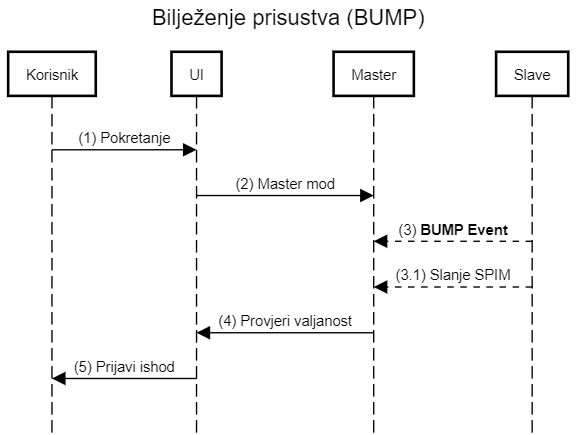
\includegraphics[width=0.7\textwidth]{material/dia/02_bump}
    \caption{Dijagram interakcije - bilježenje prisustva studenata (Master BUMP)}
\end{figure}
\paragraph*{}
Ukoliko su ispunjeni prethodno pobrojani zahtjevi, dovoljno je da student sa podešenom Logit aplikacijom na svom uređaju prinese slave (S) uređaj master (M) uređaju i da njegovo prisustvo bude zabilježeno i prikazano na ekranu M uređaja. Samu interakciju (BUMP) inicira studentski S uređaj. Prilikom ovog BUMP događaja dolazi do razmjene kriptografski potpisanih podataka o vremenu i lokaciji (SPIM) sa S na M, gdje M vrši validaciju primljenih podataka poredeći studentsko vrijeme i lokaciju sa vremenom i lokacijom na M uređaju, gdje se prisustvo odbija ukoliko se ustanovi pokušaj lažiranja podataka.

\subsection*{Prijava prisustva}
\begin{figure}[H]
    \centering
    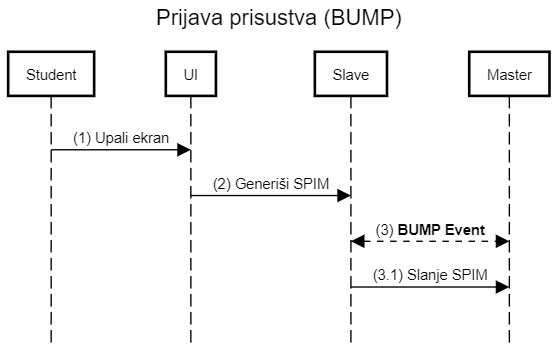
\includegraphics[width=0.7\textwidth]{material/dia/03_prijava}
    \caption{Dijagram interakcije - prijava prisustva studenta (Slave BUMP)}
\end{figure}
\paragraph*{}
Studentski S uređaj i M uređaj nastavnog osoblja podešavaju se na isti način opisan iznad, jedina praktična razlika javlja se prilikom korištenja, gdje je za S uređaj čije se prisustvo bilježi dovoljno upaliti ekran uređaja da bi se mogla ostvariti BUMP interakcija prislanjanjem S na M. Ovo je moguće jer se NFC HCE emulator Logit aplikacije izvršava u pozadini Android sistema.

\subsection*{Pohranjivanje potpisa sesije na LAPI}
\paragraph*{}
Svako bilježenje prisustva unutar Logit Android UI odvija se unutar sesije (SESS) koja se automatski započinje prilikom prvog uspješno zabilježenog prisustva i traje sve dok korisnik ne izvrši pohranu navedene sesije na LAPI servis. Klikom na SYNC dugme prikupljeni podaci šalju se LAPI servisu, provjeravaju se jedinstveni potpisi studenata te potpis ukupne sesije od strane M uređaja, ukoliko se ne pronađu nepravilnosti navedeni podaci se pohranjuju u LAPI repozitorij potpisa, takvi podaci kriptografski su osigurani od naknadne izmjene.

\begin{figure}[H]
    \centering
    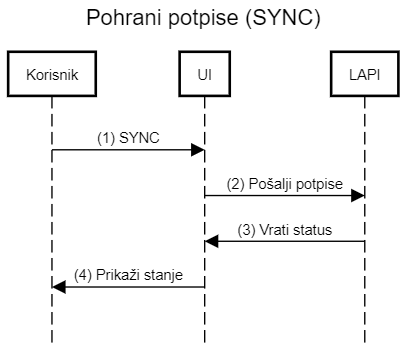
\includegraphics[width=0.6\textwidth]{material/dia/04_sync}
    \caption{Dijagram interakcije - pohranjivanje potpisa na LAPI (SYNC)}
\end{figure}
\paragraph*{}
Potpisi pohranjeni u LAPI repozitoriju mogu dalje biti korišteni u integrisanim aplikacijskim rješenjima koja zahtijevaju ovakvu vrstu podataka pomoću ponuđenog LAPI REST interfejsa, te se mogu smatrati relevantnim i sigurnim dokazom prisustva.

\section{Tehnički model rješenja}
\paragraph*{}
Uvodi se dodatno pojam lokacijskog dokaza\cite{locproof} koji u širem smislu u kontekstu podređenog korisnika (en. slave), obuhvata kriptografski potpisan korisnički identitet, korisnički uređaj, vrijeme i GPS lokacijske podatke korisničkog uređaja. Za svrhu osiguranja jedinstvenosti identiteta i vjerodostojnosti potvrde lokacijskih dokaza odabrano je korištenje RSA asimetrične enkripcije, gdje se pri uspješnoj autentifikaciji generiše jedinstveni set ključeva za korisnički uređaj, privatnom dijelu ključa nije moguće pristupiti izvan aplikacije (SEC1), niti je moguće eksportovati ključ (SEC2), a u određenom vremenskom period može postojati samo jedan valjan set ključeva za jednog korisnika jer se raniji ključevi ne uzimaju u obzir ukoliko postoji noviji set (SEC3), sprječavajući tako replikaciju identiteta na više uređaja.

\paragraph*{}
Pored Android komponente aplikacije (UI) izrađena je i serverska aplikacija u programskom jeziku Python (LAPI), čija je namjena posredovanje u komunikaciji sa autentifikacijskim agentom (ZAMGER), te pohranjivanja i održavanje javnih korisničkih kriptografskih ključeva (CERT) i njihovo povezivanje sa autentifikacijskim podacima korisnika, pored toga služi i kao repozitorij za potpisana prisustva (ATTN). Na ovu komponentu se može gledati kao na integrisani namjenski repozitorij korisničkih certifikata i domenski repozitorij neporecivih i neizmjenjivih lokacijskih dokaza (SPIM).

\paragraph*{}
Budući da na Elektrotehničkom fakultetu u Sarajevu postoji SSO (en. Single-Sign On) politika autentifikacije, u serverskoj komponenti (LAPI) je implementiran autentifikacijski posrednik koji prilikom prvog pokretanja aplikacije prijavljuje korisnika koristeći postojeće pristupne podatke, tom prilikom u slučaju uspješne prijave generiše se i jedinstveni set RSA ključeva dužine 2048 bita (KEYS), koji se pohranjuju na korisničkom uređaju (DEVICE), a javni dio, tj. certifikat (CERT) se pohranjuje i u repozitorij ključeva (LAPI) sa poveznicom na korisnički identitet, kasnije se ti certifikati koriste za provjeru valjanosti potpisa lokacijskih dokaza (SPIM).

\paragraph*{}
Da bi se osigurala jednostavnost korištenja aplikacije odabrana je implementacija HCE emulacijskog načina rada NFC komunikatora koji omogućava korisniku da izvrši komunikaciju sa drugim uređajem bez potrebe da pokreće aplikacijski prozor na svom uređaju, dovoljno je da upali ekran svoj uređaja i prinese ga master (M) uređaju koji prikuplja potpise, u ovom slučaju drugoj instanci Logit aplikacije na kojoj je pokrenuta aktivnost za prikupljanje potpisa (LAPP).

\paragraph*{}
Približavanjem mobilnih uređaja (BUMP) otvara se jednosmjerni komunikacijski kanal u smijeru od slave (S) prema master (M) uređaju korištenjem ISO/IEC 14443 Tip A komunikacijskog protokola pri čemu se emulira NFC Forum Tag tipa 4 i putem NDEF Aplikacije prenosi jedna NDEF poruka (NDEFMSG) koja sadrži vremensko-lokacijski dokaz potpisan od strane korisnika, nadalje u tekstu označen kao SPIM (en. spime)\cite{bruces}.

\paragraph*{}
Po primitku poruke nadređeni uređaj (en. master) koji osluškuje da mu se pridruže podređeni uređaji (en. slave) i ima pokrenutu Logit aplikaciju, tu poruku sprema u lokalni repozitorij potpisa ukoliko ona zadovolja uslove da očitana slave GPS lokacija nije udaljena više od 50 metara od očitane master GPS lokacije (VK1 - validacijski kriterij \#1), te da podešena razlika satova master i slave uređaja nije veća od 300 sekundi (VK2), bez da nad SPIM objektom vrši ikakve izmjene, ukoliko SPIM objekat ne zadovoljava date validacijske kriterije odbija se i ispisuje se odgovarajuća poruka na master ekranu. Moguće je naknadno klikom na validacijsko dugme (ACTVAL) u korisničkom interfejsu izvršiti provjeru svih prikupljenih potpisa tokom jedne sesije (SESS), tom prilikom se, ukoliko postoji mrežna veza; svi potpisi pošalju Logit serveru (LAPI) na provjeru i vraća se stanje valjanosti potpisa za sve proslijeđene SPIM objekte.

\paragraph*{}
Ukoliko master (M) želi da pohrani SPIM objekte iz jedne sesije (SESS) na Logit server (LAPI), klikom na sinhronizacijsko dugme u interfejsu (ACTSYNC), on vrši dodatno potpisivanje svakog SPIM objekta svojom komponentom privatnog ključa (MPRK), tako što potpiše hash (SHA256) vrijednost SPIM objekta (AID) sa dodatim svojim jedinstvenim master korisničkim imenom (MUSER) i jedinstvenim identifikatorom sesije (SID) i dodatno generiše SHA256 vrijednosti tih potvrda (CID), nakon čega objedinjuje sve CID vrijednosti i dodatno ih potpisuje svojim MPRK, sve te vrijednosti šalje Logit server (LAPI) na pohranjivanje, ovakvom procedurom se obezbjeđuje neporecivost i neizmjenjivost SPIM i SESS objekata, jer onemogućava izmjene pojedinačnih SPIM objekata, te brisanje ili dodavanje objekata u finaliziranoj sesiju (SESS) od strane malicioznih aktera bez da naruši integritet SHA256 vrijednosti.

\paragraph*{}
Uzmimajući u obzir bitnost rješenja i visoku vjerovatnoću svakodnevne primjene kod ciljane korisničke grupe, te izazove koje takav slučaj korištenja predstvalja omogućena je i direktna e-mail komunikacija za prijavu grešaka ili slanje prijedloga sa glavnog korisničkog interfejsa (ACTBUG). Kako se radi o slojevitom i kompleksnom softverskom rješenju za više detalja referirati se na izvorni kod priložen u dodatku.

\begin{figure}[H]
    \centering
    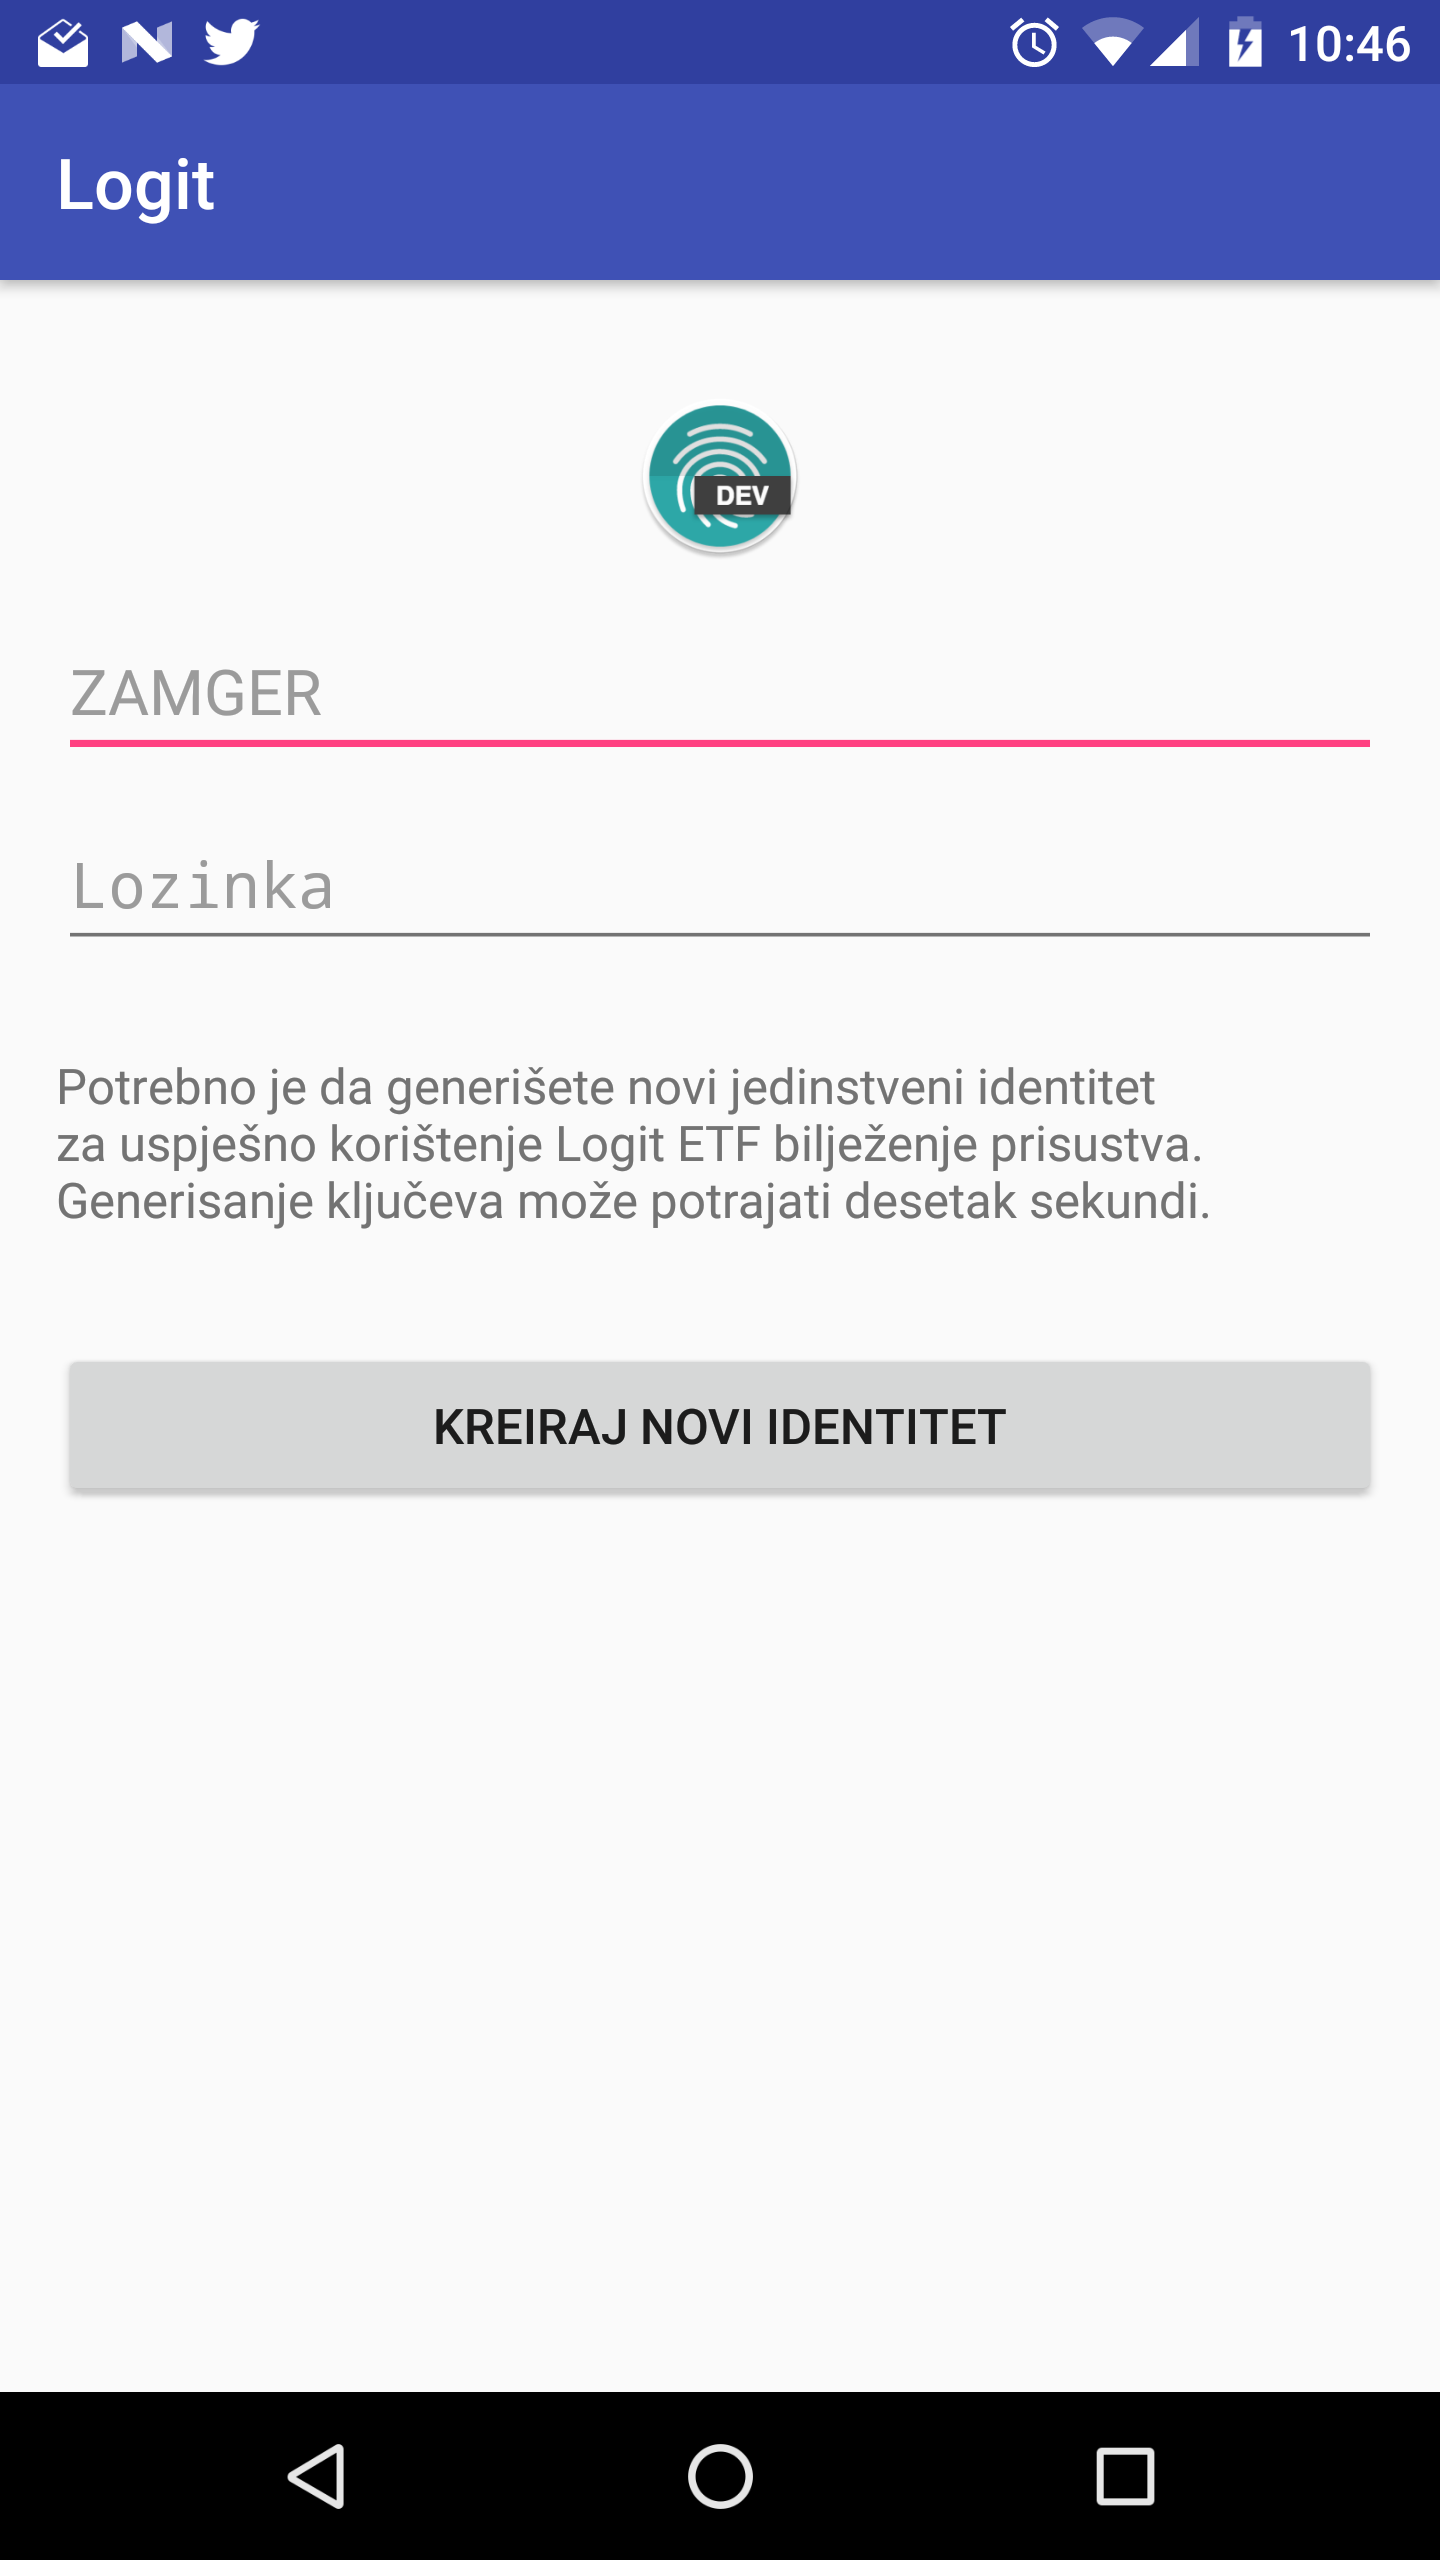
\includegraphics[width=0.45\textwidth]{material/00-login}
    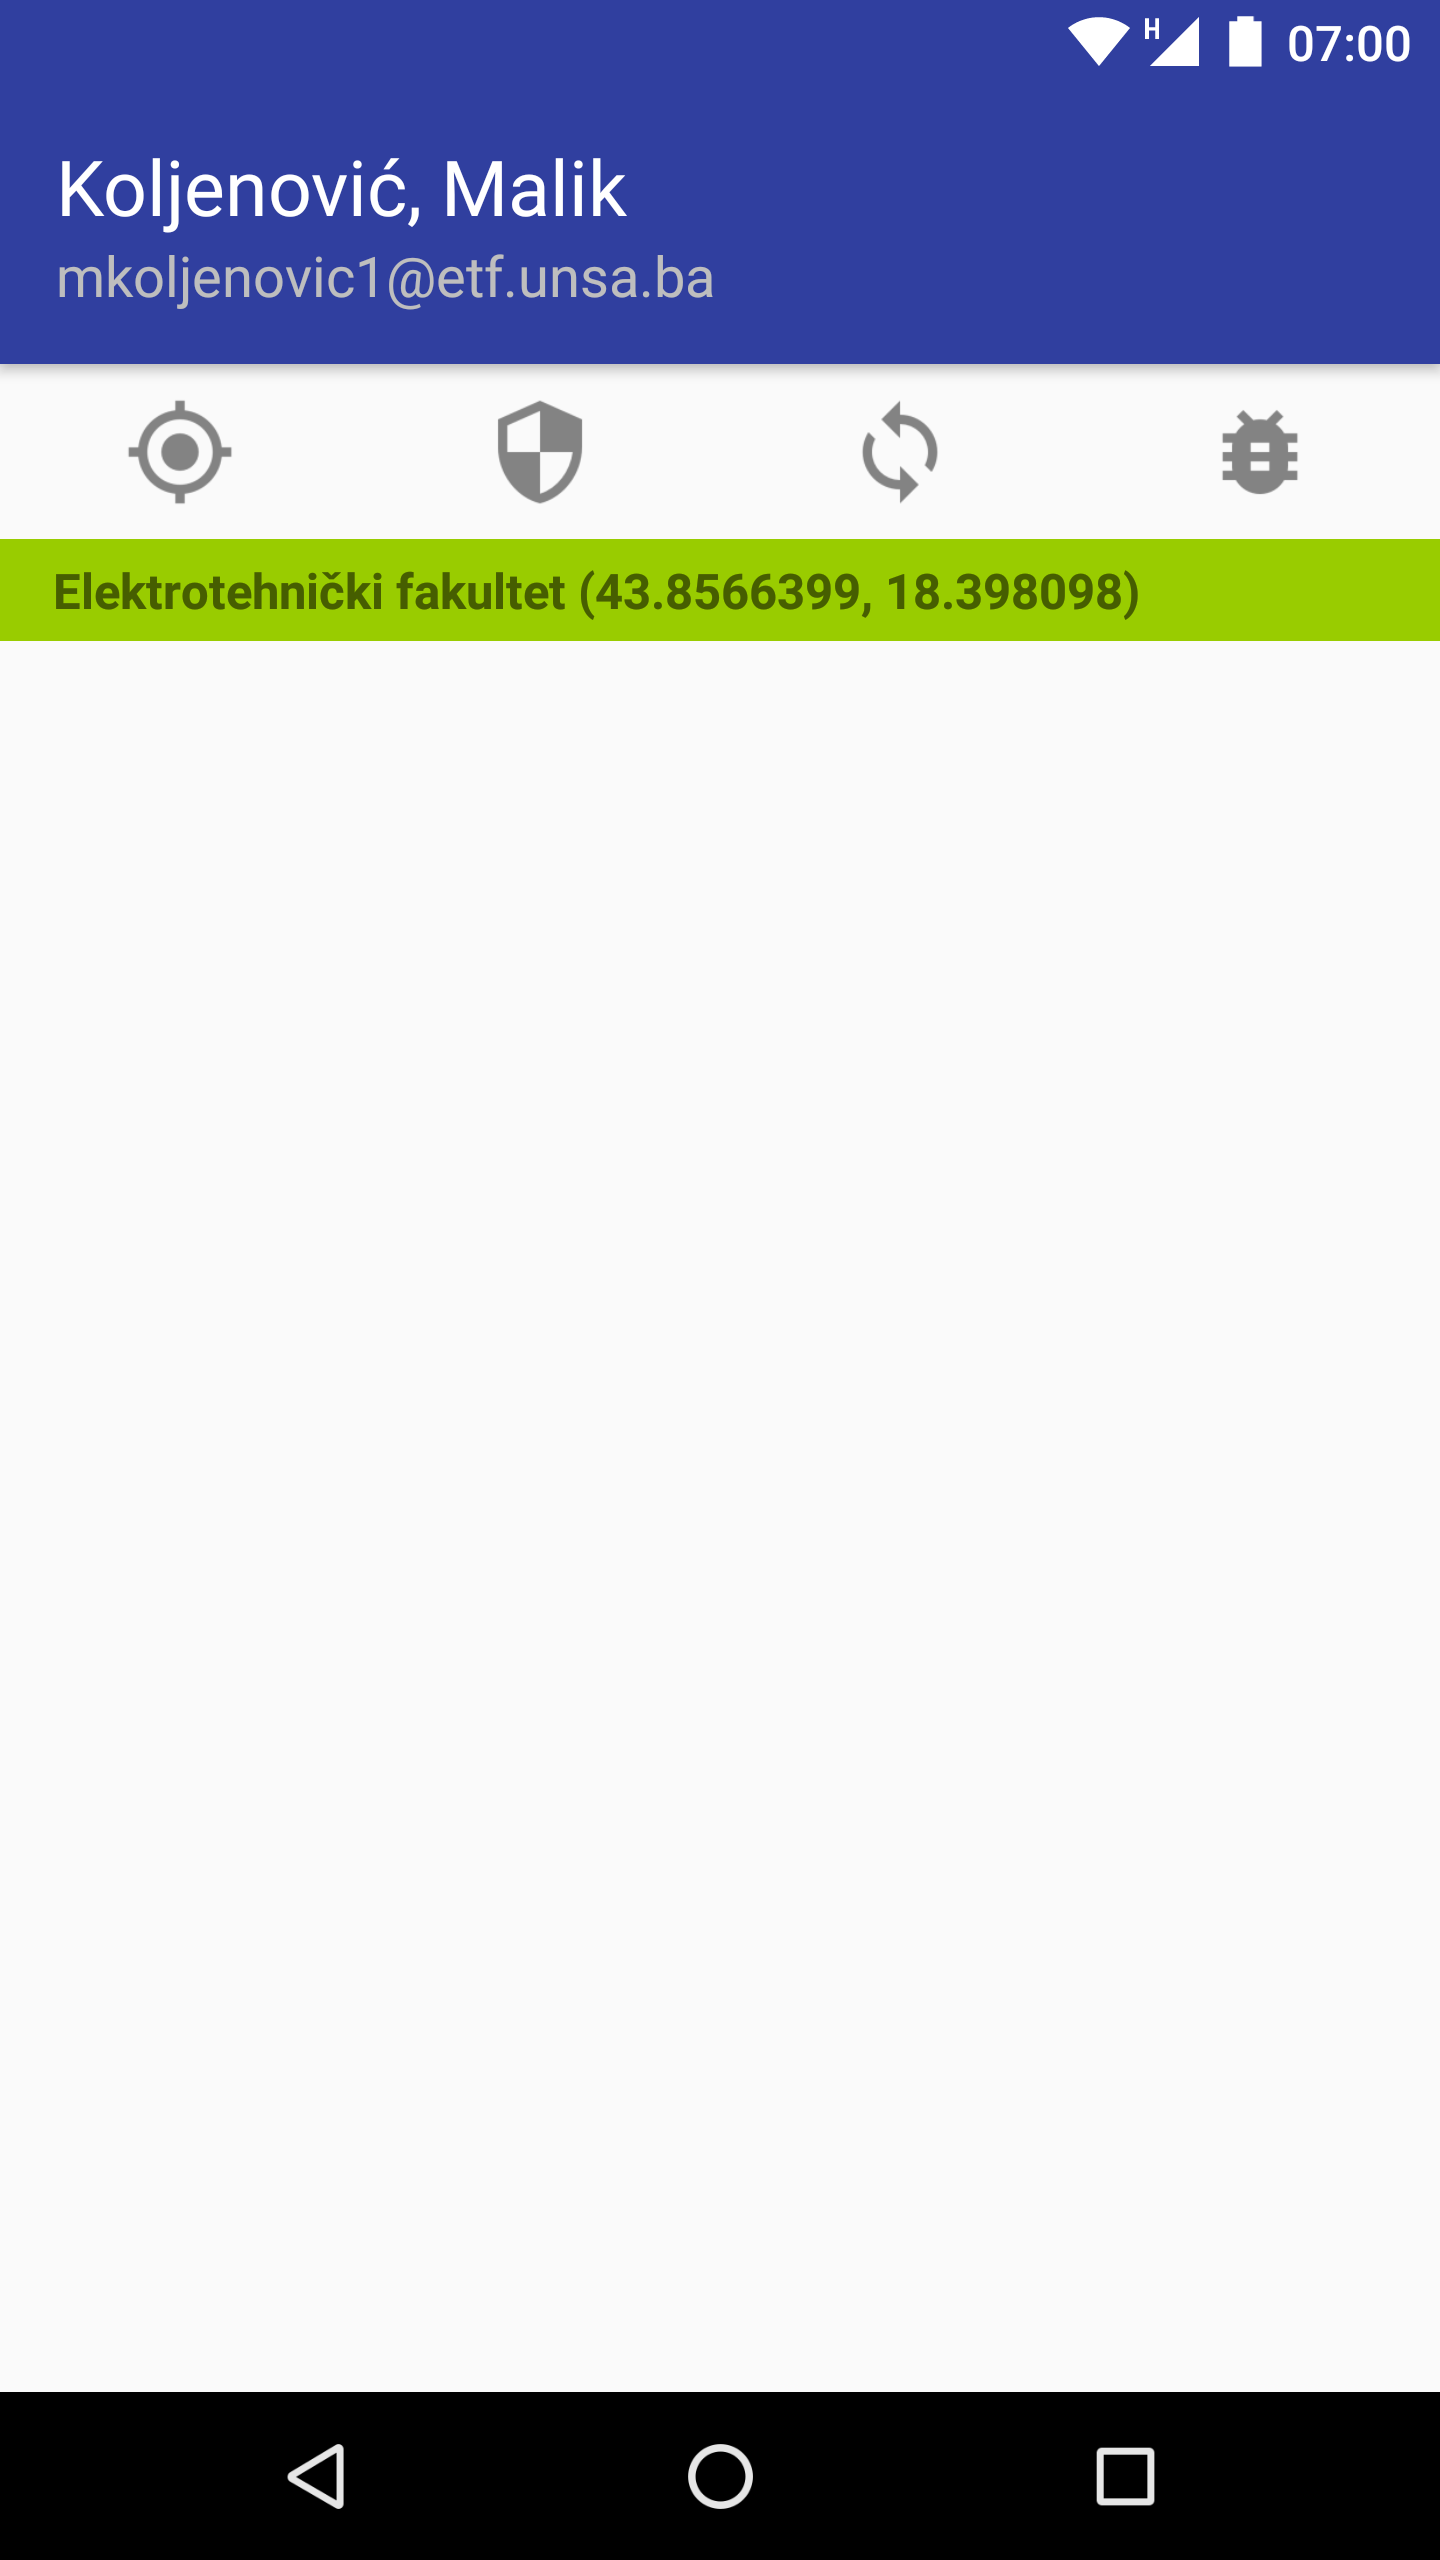
\includegraphics[width=0.45\textwidth]{material/01-attendance}
    \caption{Logit UI Android prikaz korisničkog interfejsa}
\end{figure}